
\lettrine[lines=3]{P}{}rocedurally generating 3D models of plant-life is a challenging task, largely due to the complex branching structures and variation between different types of plant species. Up until recently all assets within 3D graphics applications either had to be scalpted by hand using a 3D modeling software, or scanned using photogrammetry, laser triangulation or some form of contact based 3D scanning. These methods are still used today but tend to be very time consuming and extremely costly. With the increase in computational power over the last few decades more emphasis has been placed on the use of produral generation to create complex structures such as tarrain, architecture, sound, character models and weaponry with far greater speed than previous techniques and often much better realism than would be possible with artists, however, plant-life still stands as a challenge as there are so many possible species, that it becomes difficult to define a system that can represent them all in a way that is simple, understandable and accurate. The Lindenmayer System (L-system) stands as a solution to this problem, it was originally developed by Aristed Lindenmayer as a way to represent the development of multicellular organisms \cite{lindenmayer1968mathematical}, but has since gained popularity in the area of procedural generation and has been adapted to represent different types of structures, mainly for plant-life, such as trees, flowers, algea and grasses. The L-system has also been used to represent non-organic structures such as music, artificial neural networks and tiling patterns \cite{Prusinkiewicz1989}. The L-system in its most basic form, is a formal grammar which contains a set of symbols that belong to an \textit{alphabet}, the alphabet is used to create a starting string known as the \textit{axiom} and a set of production rules. The production rules are applied to each symbol in the axiom which dictates whether or not the symbol can be rewriten, and furthermore what they will be rewritten with. In essence, the L-system uses the set of production rules to generate a resulting string of symbols which follow those production rules. The resuting string can then be interpreted in a way that best fits what it is representing, for example a model of a plant. \\

This thesis develops upon the L-system concepts described by Przemyslaw Prusinkiewicz and Aristid Lindenmayer to procedurally generate structures of plant-life in real-time, the L-system grammar allows the specification of the structure of a plant to be described in a human readable, formal grammar, and to specify variation in shape, size and branching structure within a particular species. Furthermore, this thesis will also investigate the use of a parameterised L-systems to provide physical properties using string rewriting, which in turn will enable the animation and physical behaviour of the plant it generates, thus making it possible to simulate external forces such as gravity and wind.

\section{Introduction to Procedural Generation}

Procedural generation is used in many different areas and applications in computer graphics, particularly when generating naturally occuring structures such as plants or terrain. An effective procedural generator is capable of taking input in the form of a relatively simple description of what it should be generating, its job is then to computationally generate the structure in a way that is accurate to the description given. Currently there are three main methods for procedurally generating models of plant-life, these are genetic algorithms \cite{haubenwallner2017shapegenetics}, space colonisation algorithms\cite{juuso2017procedural} and the L-system. The genetic algorithm and space colonisation algorithms are similar in that they require the overall shape of the plant to be described by simple 3D shapes, the algorithm then creates a branching structure that matches the simple 3D description. The limitation of these methods is that the 3D description is not very specific and although it can get good results for trees, it may not be able to generate a different type of plant-life, such as flowers. Plant-life can have very complex and seemingly random structures, however, with closer observation, trees of a similar species have obvious traits and features, for instance a palm tree (Arecaceae) has long stright trunks with leaves exclusively near the top, the leaves are long, compound leaves, branching in all different directions. Comparatively a pine tree has a long staight trunk with many branches coming off in different directions pupendicular to the ground, from its base to the top of the trunk. These are two very different species of trees and look quite different, however they share very similar properties. The challenge behind procedurally generating and simulating trees is how to provide a human readable grammar that describes in sufficient detail, how it should generate and render the three dimensional model, whilst allowing for randomness and variety within the generation process. It must be relatively straightforward and intuitive to define the procedural generation description, and must accurately represent it, furthermore, the description must be able to fit many different species of trees with varying characteristics, and must not be limited to only known species of trees, as some graphics applications may require something that is other-wordly.

\section{Introduction to Rewriting Systems}

String rewriting also known as rewrite systems are the fundamental concept behind L-systems. In their most basic form, rewrite systems are a set of symbols or states, and a set of relations or production rules that dictate how to transform from one state to the other \cite{prusinkiewicz2012algorithmic}. Using these state transitions it is possible to generate complex structures by successively replacing parts of a initial simple object with more complex parts. Rewrite systems can be non-deterministic, meaning that there could be a transition that depends on a condition being met or on a neighbouring states. Using this rewriting concept any preceeding state can rely upon the current state as well as any conditions neccessary for transformation, if neither of these are met the state will remain the same, and will be checked in the next rewriting stage. A graphical representation of an object defined in rewriting rules can be seen below in figure \ref{snowflake curve} below, called the snowflake curve proposed by Von Koch \cite{koch1906methode}.

\begin{figure}[htbp]
	{\centering
		\setlength{\fboxrule}{1pt}
		\vspace{7px}
		\fbox{
			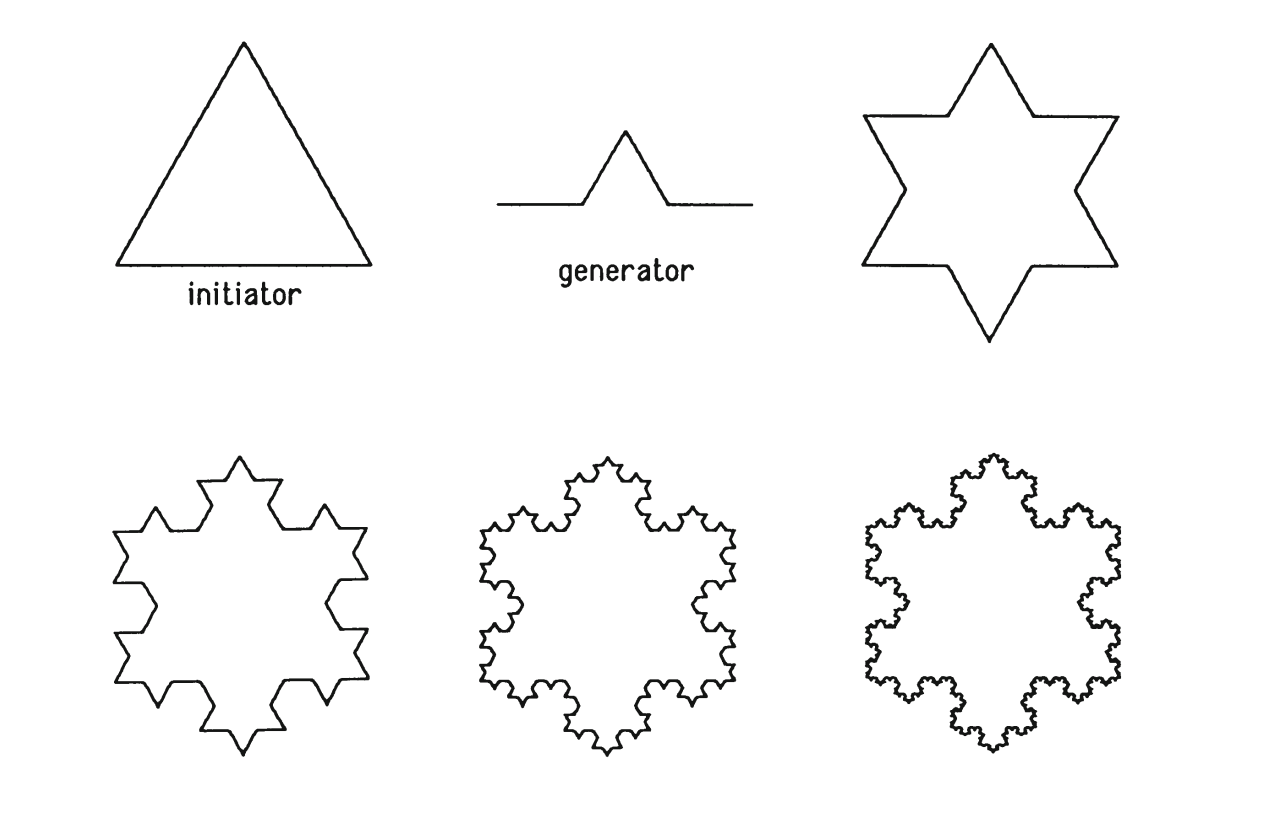
\includegraphics[scale=0.3]{Diagrams/snowflakeCurve.png}
		}
		\caption{Construction of the snowflake curve\cite{prusinkiewicz2013lindenmayer}.} \label{snowflake curve}
	}
\end{figure}
\FloatBarrier

The snowflake curve shown in figure \ref{snowflake curve} above, starts with two parts the initiator which is the initial set of edges forming a certain shape, and the generator which is a set of edges. The generator replaces each edge of the initiator forming a new shape, that new shape then becomes the new initiator where each edge is again replaced by the generator, and so on. The result is a complex shape similar to that of a snowflake. The initiator, generator concept can be adapted and represented as a set of strings capable of producing a similar result.

\section{Introduction to Grammars}

In the context of computer science, grammars are defined as a set of rules governing which strings are valid or allowable in a language or text. They consist of syntax, morphology and semantics. Formal languages have been defined in the form of grammars to suit particular problem domains. It is natural for humans to communicate a problem or solution in the form of language, it is therefore intuitive to use a language to describe the desired outcome when dealing with the procedural generation of plant-life. In the past, formal grammars have been used extensively in computer science in the form of programming languages in which humans can provide a computer with a set of instructions to carry out in order to gain an expected result. The challenge is therefore to create a  grammar in the form of a rewriting system that facilitates the procedural generation of plant-life. A rewriting system such as the L-system operates in a way that is consistant with a context-free class of Chomsky grammar \cite{chomsky1956three}, similar to that of the programming language ALGOL-60 introduced by Backus and Naur in  1960\cite{backus1960report}. In figure \ref{chomsky grammars} below, there are two types of L-system grammars that overlap the classes of chomsky grammars, the OL-system and the 1L-system. The details of these two systems will be discussed in detail chapter \ref{l-system chapter}, but in summary, 0L-systems are grammars that can represent a context-sensitive Chomsky grammar but generally tend to be context-free, the main difference between the 0L-system and the 1L-system is that 1L-systems can be recursively enumerable. Furthermore, it is possible for a 1L-system to represent any 0L-system, therefore, 1L-system languages tend to be more complex and verbose when compared to 0L-systems, this creates a trade off between a more powerful and complex language or a less powerful but simpler language. 

\begin{figure}[htbp]
	{\centering
		\setlength{\fboxrule}{1pt}
		\vspace{7px}
		\fbox{
			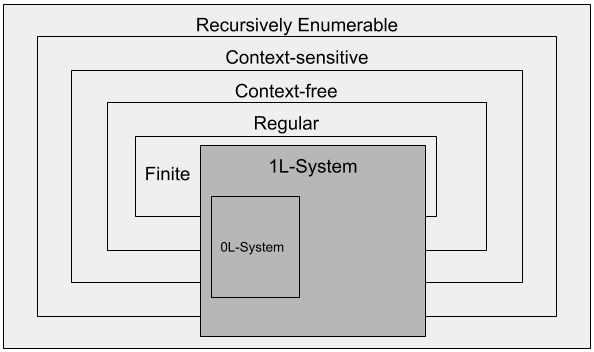
\includegraphics[scale=0.5]{Diagrams/ChomskyGrammar.png}
		}
		\caption{Diagram of the Chomsky hierarchy grammars with relation to the 0L and 1L systems generated by L-systems.} \label{chomsky grammars}
	}
\end{figure}
\FloatBarrier

\section{Motivations}
 

One of the most time consuming parts for digital artists and animators is creating differing variations of the same piece of artwork. In most games and other graphics applications environment assets such as trees, plants, grass, algae and other types of plant life make up the large majority of the assets within a game, and creating a plant asset can take a skilled digital artist more than an hour of work by hand, The artist will often have to create many variations of the same asset in order to obtain enough variation that a user of that graphics application would not notice that the asset has been duplicated, if this is multiplied by the number of assets that a given artist will have to create or modify, there is an incredible number of hours that could have potentially been put to use creating much more intricate assets. In addition to this, it is also important to note that graphics assets are then stored in large data files, describing the geometry and textures and other information. If we require three very similar plants, we have to store three separate sets of data. Procedurally generating plants can avoid this wasteful data storage entirely, instead a relatively small L-system description can be stored which can be used to procedurally generate all the required geometry and other information during the execution of the program.\\

The L-system can not only procedurally generate the geometry of the plant-life but can also generate parameters physical properties of the plant inself such as the weight and flexibility of branches as well as its wind resistance and many other important information that can be used to simulate or animate the motion of the plant under various forces. 

\section{Structure of Thesis}

This thesis is split into three major parts. Part 1 focuses on the L-system itself, it defines the various types of L-systems for modeling plant-life, the concept of a parametric L-system as well as some techniques for definiting randomness and stochasticisity within an L-system in order to create variaty. Part 2 talks about the L-system rewriter implementation, covering how the L-system generates the resulting string and structures relavant rendering. Part 3 focuses on the interpretation and renderer implementation and how to render a convincing model of a tree on the screen, as well as simulation and animation of the generated plants.





